\chapter{रक्तचाप का नियमन और व्यायाम}\label{ch:b2:blood-pressure}

लेटने के बाद जल्दी से खड़े होइए और, एक सेकंड के लिए, आधा लीटर
\omterm{def:b2:blood-circulation:blood}{रक्त} आपकी टाँगों की \omterm{def:b2:blood-circulation:vessels}{शिराओं} में बह जाता है; \omterm{def:b2:heart:anatomy}{हृदय}, कम पाकर,
कम पंप करता है, सिर पर दाब गिरता है, और मस्तिष्क --- जो
\omterm{def:b2:heart:anatomy}{हृदय} से \qty{40}{cm} ऊपर है और ऑक्सीजन संचित नहीं कर सकता --- मूर्छा से
सेकंड-दो सेकंड दूर रह जाता है। वह लगभग कभी मूर्छित नहीं होता, क्योंकि एक ही धड़कन के भीतर
कोई प्रतिवर्त \omterm{def:b2:blood-circulation:vessels}{धमनिकाएँ} कस चुका होता है और \omterm{def:b2:heart:anatomy}{हृदय} तेज़ कर चुका। किसी बस के
लिए दौड़िए और पेशियों को विश्राम के मुक़ाबले दस गुना \omterm{def:b2:blood-circulation:blood}{रक्त} चाहिए;
वह उन्हें मिनट भर के भीतर मिल जाता है, और जो दाब उसे चलाता है वह
स्थिर रखा जाता है जबकि पूरी देह का प्रतिरोध दो
तिहाई गिर जाता है। यह अध्याय उसी नियमन के बारे में है: दाब क्या
तय करता है, उसे कैसे भाँपा जाता है, वह तेज़ प्रतिवर्त तथा वे धीमे हॉर्मोन
जो उसे सुधारते हैं, और व्यायाम उस तंत्र को कुचलने के बजाय कैसे
फिर से गढ़ देता है।

\section{वह दाब है क्या}

\begin{theorem}[परिसंचरण का समीकरण]\label{thm:b2:blood-pressure:equation}
\index{माध्य धमनीय दाब}\index{कुल परिधीय प्रतिरोध}
\omterm{thm:b2:blood-pressure:equation}{माध्य धमनीय दाब} $\bar P$ उसका गुणनफल है जो \omterm{def:b2:heart:anatomy}{हृदय}
भीतर डालता है और जो वाहिकाएँ बाहर जाने देती हैं:
\[
\bar P - P_{\text{शिरा}} = Q\,R, \qquad Q = f\times V_s,
\]
जिसमें $Q$ \omterm{thm:b2:heart:starling}{हृद्-निर्गम} है (हृद्-दर $f$ गुणा \omterm{prop:b2:heart:cycle}{आघात-आयतन}
$V_s$), $R$ \omterm{thm:b2:blood-pressure:equation}{कुल परिधीय प्रतिरोध} --- यानी सारे
अंगों की \omterm{def:b2:blood-circulation:vessels}{धमनिकाएँ} समांतर में --- और $P_{\text{शिरा}}$ शिरीय दाब,
जो शून्य के पास है। विश्राम में, $\qty{5}{L/min}\times\qty{1.08}{mmHg.s/mL}$
\qty{90}{mmHg} देता है। दाब का हर नियमन तीन
राशियों में से एक पर काम करता है: वह दर, वह \omterm{prop:b2:heart:cycle}{आघात-आयतन}
(\cref{ch:b2:heart} के भरने तथा सुकुंचनशीलता से) या वह प्रतिरोध
(धमनिका-त्रिज्या से, चौथी घात तक)। चूँकि वे अंग समांतर में हैं,
इसलिए हर एक को प्रवाह उस दाब में उसका हिस्सा बँटा
उसका अपना प्रतिरोध है: किसी एक अंग की \omterm{def:b2:blood-circulation:vessels}{धमनिकाएँ} फैलाना उसका
प्रवाह बाक़ियों को बदले बिना चढ़ा देता है, बशर्ते वह दाब थमा रहे ---
और दाब थामना ही उस नियमन का काम है।
\end{theorem}
\begin{proof}
किसी तरल के लिए ओम का नियम: किसी प्रतिरोध से होकर प्रवाह उसके आरपार
दाब-पात बँटा वह प्रतिरोध है (प्वाज़ेई,
\cref{ch:b2:blood-circulation}); समांतर में प्रतिरोधों के लिए
प्रवाह जुड़ते हैं और $1/R = \sum 1/R_i$। किसी धड़कन भर माध्य दाब
लगभग अनुशिथिलनी धन \omterm{thm:b2:blood-circulation:windkessel}{स्पंद दाब} का एक तिहाई है:
$80 + 40/3 = \qty{93}{mmHg}$।
\end{proof}

\begin{omfigure}
\begin{tikzpicture}[every node/.style={font=\scriptsize}, >=stealth]
  \node[draw, rounded corners, fill=omThm!15, minimum width=2.4cm, minimum height=1cm, align=center] (heart) at (0,0) {हृदय\\$Q = f\,V_s$};
  \draw[very thick, omThm] (1.2,0) -- (2.4,0);
  \draw[very thick, omThm] (2.4,-2.4) -- (2.4,2.4);
  \foreach \y/\org/\r in {2.0/{मस्तिष्क}/{$R_1$}, 1.0/{हृद्-पेशी}/{$R_2$}, 0/{आँत और यकृत}/{$R_3$}, -1.0/{वृक्क}/{$R_4$}, -2.0/{पेशी, त्वचा}/{$R_5$}} {
    \draw[very thick, omThm] (2.4,\y) -- (3.6,\y);
    \draw[thick, decorate, decoration={zigzag, segment length=4pt, amplitude=2pt}] (3.6,\y) -- (5.0,\y);
    \node[above] at (4.3,\y+0.05) {\org};
    \node[below] at (4.3,\y-0.05) {\r};
    \draw[very thick, omDef] (5.0,\y) -- (6.2,\y);
  }
  \draw[very thick, omDef] (6.2,-2.4) -- (6.2,2.4);
  \draw[very thick, omDef] (6.2,0) -- (7.4,0) |- (0,-3.2) -- (0,-0.5);
  \node[omThm, above] at (1.8,0.05) {$\bar P$};
  \node[omDef, below] at (3.7,-3.2) {शिराएँ, $P_{\text{शिरा}} \approx 0$};
  \node[anchor=west, align=left] at (7.8,1.5) {समांतर में अंग:\\$1/R = \sum 1/R_i$\\अंग $i$ को प्रवाह: $\bar P/R_i$};
\end{tikzpicture}

{\small किसी परिपथ के रूप में परिसंचरण: एक पंप, एक दाब, और
समांतर में अंगों के धमनिका-प्रतिरोध। हर अंग
$\bar P/R_i$ लेता है; और वह नियमन $\bar P$ थामे रहता है जबकि $R_i$
माँग के अनुसार समंजित होते हैं।}
\end{omfigure}

\begin{proposition}[दाब को नियंत्रित क्यों करना पड़ता है]\label{prop:b2:blood-pressure:why}
बहुत नीचा हो, और मस्तिष्क --- जो किसी खड़े वयस्क में \omterm{def:b2:heart:anatomy}{हृदय} से \qty{40}{cm}
ऊपर है, जिसका दाम द्रवस्थैतिक शीर्ष का \qty{31}{mmHg} है --- तथा
हृद्-पेशी स्वयं कम सींची जाती है: मस्तिष्क सेकंडों में
चूक जाता है। बहुत ऊँचा हो, और वाहिकाएँ क्षतिग्रस्त होती हैं: धमनी-भित्ति
मोटी तथा कड़ी हो जाती है, वृक्क के केशिकागुच्छ छिल जाते हैं, दृष्टिपटल
से \omterm{def:b2:blood-circulation:blood}{रक्त} बहता है, और \omterm{def:b2:heart:anatomy}{हृदय} उस दाब के विरुद्ध तब तक जूझता है जब तक चूक न जाए।
उस दाब को तब भी स्थिर रहना है जब अंगों की माँगें
परिमाण की एक कोटि भर बदलें --- भोजन के बाद आँत, व्यायाम में पेशियाँ,
गर्मी में त्वचा --- और जब रक्त-आयतन स्वयं
किसी रक्तस्राव या पसीने में खो जाए। दो तंत्र यह करते हैं: कोई तंत्रिका
प्रतिवर्त जो एक धड़कन के भीतर उस दर, \omterm{prop:b2:heart:cycle}{आघात-आयतन} तथा
प्रतिरोध पर काम करता है, और वे हॉर्मोन तंत्र जो घंटों तथा दिनों भर
उस प्रतिरोध पर और, सबसे बढ़कर, वृक्क से होकर रक्त-आयतन पर काम करते
हैं।
\end{proposition}

\begin{omfigure}
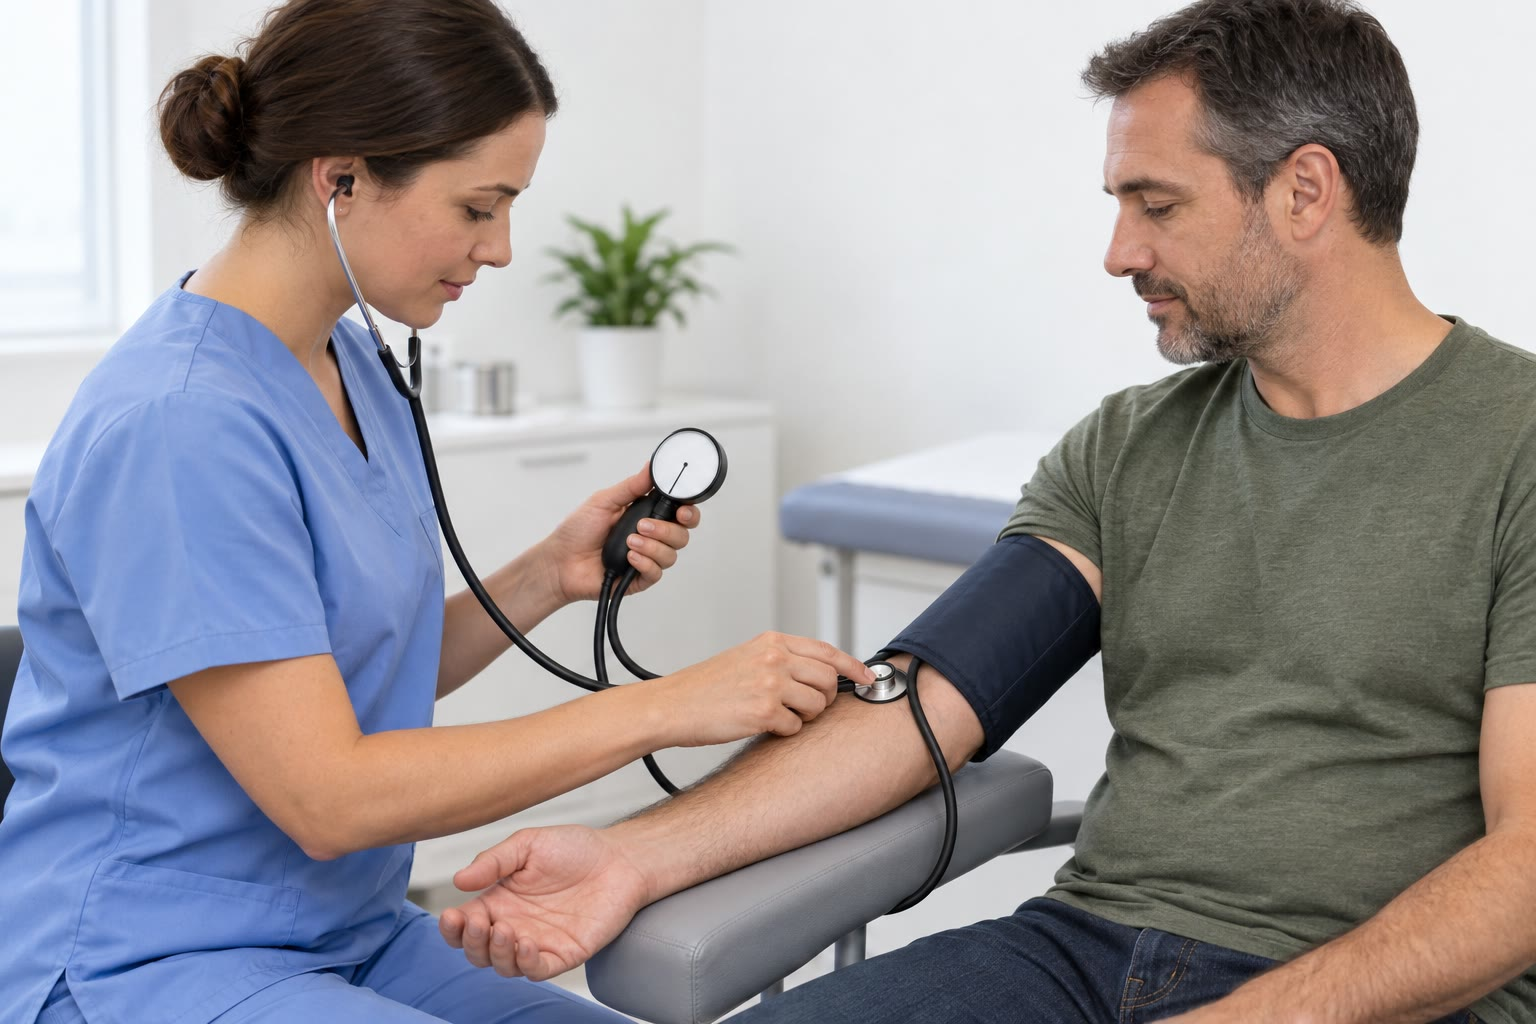
\includegraphics[width=0.6\linewidth]{images/book4/ai/b4-18-blood-pressure-cuff.jpg}

{\small दाब मापना। वह पट्टी प्रकुंचनी दाब से ऊपर तक फुलाई जाती है,
ताकि कोई \omterm{def:b2:blood-circulation:blood}{रक्त} न गुज़रे; और ज्यों-ज्यों वह छोड़ी जाती है, त्यों-त्यों
आलोचित्र के नीचे विक्षुब्ध प्रवाह की पहली ध्वनियाँ
प्रकुंचनी दाब अंकित करती हैं, और उनका लोप, जब वह \omterm{def:b2:blood-circulation:vessels}{धमनी} पूरे चक्र भर
खुली रहती है, अनुशिथिलनी दाब।}
\end{omfigure}

\section{तेज़ पाश: दाब-प्रतिवर्त}

\begin{definition}[दाब-प्रतिवर्त]\label{def:b2:blood-pressure:baroreflex}
\index{दाबग्राही}\index{दाब-प्रतिवर्त}\index{वाहिकाप्रेरक केंद्र}\index{स्वायत्त तंत्रिका तंत्र}
ग्रीवा ज्यावों (हर ग्रीवा \omterm{def:b2:blood-circulation:vessels}{धमनी} के काँटे पर, जबड़े के नीचे) तथा
महाधमनी-चाप की भित्तियों में खिंचाव-ग्राही --- यानी
\emph{दाबग्राही} --- ऐसी दर पर दगते हैं जो उस दाब के साथ चढ़ती है
जो उन्हें फुलाए, और किसी चढ़ते दाब के लिए तेज़। उनकी तंत्रिकाएँ
मेडुला के \emph{हृद्-वाहिका केंद्रों} तक पहुँचती हैं, जो
स्वायत्त बहिर्वाह की दोनों शाखाएँ नियंत्रित करते हैं: वेगस, जिसकी
ऐसिटिलकोलीन \omterm{prop:b2:heart:conduction}{साइनु-अलिंद गाँठ} धीमी करती है, और अनुकंपी
तंत्रिकाएँ, जिनकी नॉरऐड्रिनैलिन उस गाँठ को तेज़ करती है, उस
\omterm{def:b2:heart:anatomy}{निलय} को मज़बूत करती है, \omterm{def:b2:blood-circulation:vessels}{धमनिकाएँ} सिकोड़ती है ($R$ चढ़ाकर) और
\omterm{def:b2:blood-circulation:vessels}{शिराएँ} सिकोड़ती है (संचित \omterm{def:b2:blood-circulation:blood}{रक्त} को \omterm{def:b2:heart:anatomy}{हृदय} की ओर भींचकर और वह
भरना चढ़ाकर)। दाब में कोई चढ़ाई दाबग्राही दगना बढ़ा देती है, जो
वेगस को उत्तेजित और अनुकंपी बहिर्वाह को संदमित करता है: वह दर
गिरती है, \omterm{def:b2:blood-circulation:vessels}{धमनिकाएँ} ढीली होती हैं, दाब नीचे आ जाता है। कोई गिरावट
उलटा करती है। वह पाश \qty{95}{mmHg} के पास किसी नियत बिंदु,
लगभग एक सेकंड की देरी, और ऐसी लब्धि वाली कोई \emph{ऋण प्रतिपुष्टि} है
कि कोई विक्षोभ उसके आकार के पाँचवें भाग के भीतर तक सुधार दिया जाए:
यही कारण है कि आप खड़े होने पर मूर्छित नहीं होते।
\end{definition}
\begin{proof}[प्रमाण-सामग्री]
हेरिंग (1923) ने पाया कि ग्रीवा ज्या पर दबाने से
\omterm{def:b2:heart:anatomy}{हृदय} धीमा हुआ और दाब नीचा हुआ, और यह कि ज्या-तंत्रिका काटने से
वह अनुक्रिया मिट गई। किसी अलग की हुई ग्रीवा ज्या को नियत
दाबों पर सींचते हुए उस प्राणी का धमनीय दाब अभिलिखित करने से
उस प्रतिवर्त का सिग्मॉइड वक्र मिला: उस प्राणी का दाब गिरता है ज्यों-ज्यों
ज्या-दाब चढ़ाया जाए, और वह भी \qty{100}{mmHg} के इर्द-गिर्द तीखे ढंग से तथा
\qtyrange{60}{160}{mmHg} के बाहर थोड़ा। जिन कुत्तों की ज्या- तथा
महाधमनी-तंत्रिकाएँ दोनों काट दी गई हों वे दिनों भर कोई सामान्य माध्य दाब रखते हैं पर
मिनट-दर-मिनट वह जंगली ढंग से बदलता है --- वह प्रतिवर्त कोई बफ़र है, न कि
दीर्घकालिक स्तर तय करने वाला।
\end{proof}

\begin{omfigure}
\begin{tikzpicture}[every node/.style={font=\scriptsize}, >=stealth]
  \node[draw, rounded corners, fill=omDef!15, align=center] (bp) at (0,0) {धमनीय दाब\\$\bar P$};
  \node[draw, rounded corners, fill=omDef!15, align=center] (baro) at (4.2,0) {दाबग्राही\\ग्रीवा ज्या, महाधमनी-चाप\\दगने की दर $\uparrow$, $\bar P$ के साथ};
  \node[draw, rounded corners, fill=omProp!20, align=center] (med) at (8.6,0) {मेडुला:\\हृद्-वाहिका केंद्र};
  \node[draw, rounded corners, fill=omThm!15, align=center] (vag) at (8.6,-2.2) {वेगस $\uparrow$: दर $\downarrow$};
  \node[draw, rounded corners, fill=omThm!15, align=center] (sym) at (4.2,-2.2) {अनुकंपी $\downarrow$: दर, सुकुंचनशीलता,\\धमनिका तथा शिरा की तान $\downarrow$};
  \draw[->, thick] (bp) -- (baro); \draw[->, thick] (baro) -- (med);
  \draw[->, thick] (med) -- (vag); \draw[->, thick] (med) -- (sym);
  \draw[->, thick] (sym.west) -| (bp.south) node[pos=0.75, left, align=right] {$Q\downarrow$, $R\downarrow$:\\$\bar P\downarrow$};
  \draw[->, thick] (vag.west) -- (sym.east);
  \node[anchor=north, align=center] at (4.3,-3.2) {दाब में कोई चढ़ाई किसी गिरावट से उत्तर पाती है: ऋण प्रतिपुष्टि, एक सेकंड की देरी};
\end{tikzpicture}

{\small \omterm{def:b2:blood-pressure:baroreflex}{दाब-प्रतिवर्त}। धमनीय दाब में कोई चढ़ाई
\omterm{def:b2:blood-pressure:baroreflex}{दाबग्राही} दगना बढ़ाती है, जो मेडुला को \omterm{def:b2:heart:anatomy}{हृदय} धीमा करने और
वाहिकाएँ ढीली करने के लिए चलाती है; कोई गिरावट उलटा करती है।}
\end{omfigure}

\begin{theorem}[किसी ऋण प्रतिपुष्टि पाश की लब्धि]\label{thm:b2:blood-pressure:gain}
\index{प्रतिपुष्टि लब्धि}
यदि कोई विक्षोभ, बिना नियमन के, दाब को
$\Delta P_0$ से बदल देता, और वह पाश किसी भी विचलन $\Delta P$ का उत्तर
$-G\,\Delta P$ के किसी सुधार से दे (यानी \emph{खुले-पाश की लब्धि} $G$), तो
पाश के काम कर लेने पर जो विचलन बचा रहता है वह है
\[
\Delta P = \frac{\Delta P_0}{1 + G}.
\]
\omterm{def:b2:blood-pressure:baroreflex}{दाब-प्रतिवर्त} की $G \approx 4$ है: खड़े होना, जो
\omterm{def:b2:heart:anatomy}{हृदय} पर दाब कोई \qty{40}{mmHg} गिरा देता, उसे
\qty{8}{mmHg} गिराता है; और कोई रक्तस्राव जो दाब आधा कर देता उसे
दसवें भाग भर नीचा करता है --- जब तक वह हानि उससे आगे न निकल जाए जो कसी वाहिकाएँ और कोई
तेज़ \omterm{def:b2:heart:anatomy}{हृदय} छिपा सकते हैं। वह प्रतिवर्त किसी विक्षोभ को मिटाता नहीं;
वह उसे पाँच से बाँट देता है। और वह \emph{पुनः बैठ} जाता है: किसी नए दाब पर
घंटों थामे रखने पर \omterm{def:b2:blood-pressure:baroreflex}{दाबग्राही} अभ्यस्त हो जाते हैं और उस नए स्तर की रक्षा करते हैं, और
इसीलिए वह प्रतिवर्त उच्च रक्तचाप का इलाज नहीं कर सकता और इसीलिए दीर्घकालिक
स्तर कहीं और तय होता है।
\end{theorem}
\begin{proof}
अंतिम विचलन वह विक्षोभ धन वह सुधार है:
$\Delta P = \Delta P_0 - G\,\Delta P$, इसलिए $\Delta P(1 + G) =
\Delta P_0$। $G = 4$ के साथ, $\Delta P = \Delta P_0/5$।
\end{proof}

\begin{omfigure}
\begin{tikzpicture}
\begin{axis}[
  width=0.7\linewidth, height=5.4cm,
  axis x line=bottom, axis y line=left,
  xmin=40, xmax=180, ymin=40, ymax=160,
  xlabel={ग्रीवा ज्या में दाब (\unit{mmHg})}, ylabel={परिणामी धमनीय दाब (\unit{mmHg})},
  xlabel style={font=\small, at={(axis description cs:0.5,-0.13)}, anchor=north},
  ylabel style={font=\small},
  tick label style={font=\small}, xtick={60,100,140}, ytick={60,100,140},
  clip=false,
]
\addplot[very thick, omDef, domain=40:180, samples=80] {100 + 50*tanh((100-x)/25)};
\addplot[thick, dashed, gray, domain=40:180, samples=2] {x};
\fill[omDef] (axis cs:100,100) circle (2pt); \draw[gray] (axis cs:101,100) -- (axis cs:124,110); \node[font=\scriptsize, anchor=west] at (axis cs:125,110) {नियत बिंदु};
\node[font=\scriptsize, anchor=west, align=left] at (axis cs:46,112) {नियत बिंदु के पास\\ढाल $-G$};
\end{axis}
\end{tikzpicture}

{\small \omterm{def:b2:blood-pressure:baroreflex}{दाब-प्रतिवर्त} वक्र: वह दाब जिस पर देह बैठ जाती है जब
वह अलग की हुई ज्या किसी दिए गए दाब पर थामी जाए। नियत बिंदु पर उसका
ढाल वह लब्धि है; और \qtyrange{60}{160}{mmHg} के बाहर वह प्रतिवर्त
संतृप्त है।}
\end{omfigure}

\section{धीमे पाश: हॉर्मोन और वृक्क}

\begin{proposition}[रेनिन, ऐंजियोटेंसिन, ऐल्डोस्टेरॉन, और वह आयतन]\label{prop:b2:blood-pressure:raas}
\index{रेनिन--ऐंजियोटेंसिन तंत्र}\index{ऐल्डोस्टेरॉन}\index{प्रतिमूत्रल हॉर्मोन}\index{नैट्रियूरेटिक पेप्टाइड}
घंटों तथा दिनों भर वह दाब \emph{रक्त-आयतन} तय करता है,
और वह आयतन वृक्क। जब वह दाब या वृक्क तक पहुँचाया गया सोडियम
गिरता है, या अनुकंपी तंत्रिकाएँ दगती हैं, तब वृक्क की
\omterm{def:b2:blood-circulation:vessels}{धमनिकाओं} की कोशिकाएँ एंजाइम \emph{रेनिन} \omterm{def:b2:blood-circulation:blood}{रक्त} में छोड़ती
हैं; रेनिन किसी \omterm{def:b2:blood-circulation:blood}{प्लाज़्मा} प्रोटीन को काटकर \emph{ऐंजियोटेंसिन I} बनाता है, जिसे
फेफड़े की \omterm{def:b2:blood-circulation:vessels}{केशिकाओं} का कोई एंजाइम \emph{ऐंजियोटेंसिन II} में बदल देता है
--- यानी देह का सबसे ज़ोरदार वाहिकासंकोचक, जो मिनटों में $R$ चढ़ा
देता है, और ऐसा हॉर्मोन जो अधिवृक्क वल्कुट से
\emph{ऐल्डोस्टेरॉन} स्रवित कराता है, जो वृक्क से सोडियम, और उसके साथ
जल, अगले दिनों भर रुकवाता है। पीयूष का
\emph{\omterm{prop:b2:blood-pressure:raas}{प्रतिमूत्रल हॉर्मोन}} (वैसोप्रेसिन), जो तब छोड़ा जाता है जब \omterm{def:b2:blood-circulation:blood}{रक्त}
सांद्र हो जाए या उसका आयतन गिरे, वृक्क से सीधे जल
रुकवाता है और वाहिकाएँ भी सिकोड़ता है। और जब \omterm{def:b2:heart:anatomy}{अलिंद}
बहुत अधिक आयतन से अति-खिंच जाएँ तब वे \emph{\omterm{prop:b2:blood-pressure:raas}{नैट्रियूरेटिक
पेप्टाइड}} स्रवित करते हैं, जो वृक्क से सोडियम तथा जल निकलवाता है। इस तरह
वृक्क अंतिम पंच है: वह लीटरों निकाल या रोक सकता है,
और जो दाब वृक्क के नियत बिंदु से ऊपर बना रहे वह, दिनों भर,
आयतन की हानि से सुधार दिया जाता है --- जब तक स्वयं वृक्क का
नियत बिंदु ही न चढ़ा हो, और अधिकांश उच्च रक्तचाप वही है।
(वृक्क की अपनी मशीनरी वर्ष 3 के खंड का विषय है।)
\end{proposition}
\begin{proof}[प्रमाण-सामग्री]
गोल्डब्लाट (1934) ने किसी कुत्ते के एक वृक्क की \omterm{def:b2:blood-circulation:vessels}{धमनी} सँकरी की: वह
प्राणी दिनों के भीतर उच्च-रक्तचापी हो गया और बना रहा; और वह
कम सींचा वृक्क रेनिन छोड़ता पाया गया, तथा उसे हटाने से
वह प्राणी ठीक हो गया। जो दवाएँ ऐंजियोटेंसिन के रूपांतरण
(ACE संदमक) या उसके ग्राही को रोकती हैं वे अधिकांश
उच्च-रक्तचापियों का दाब नीचा करती हैं, और किसी उच्च-रक्तचापी
चूहा-प्रजाति से प्रतिरोपित वृक्क किसी सामान्य प्राप्तकर्ता को उच्च-रक्तचापी बना देता है।
\end{proof}

\begin{omfigure}
\begin{tikzpicture}[every node/.style={font=\scriptsize}, >=stealth]
  \node[draw, rounded corners, fill=omDef!15, align=center] (fall) at (0,0) {दाब या आयतन गिरता है;\\अनुकंपी तंत्रिकाएँ दगती हैं};
  \node[draw, rounded corners, fill=omProp!20, align=center] (renin) at (4.4,0) {वृक्क छोड़ता है\\रेनिन};
  \node[draw, rounded corners, fill=omProp!20, align=center] (ang) at (8.6,0) {ऐंजियोटेंसिन II\\(रक्त तथा फेफड़े में बना)};
  \node[draw, rounded corners, fill=omThm!15, align=center] (vc) at (8.6,-2.0) {वाहिकासंकोचन:\\मिनटों में $R\uparrow$};
  \node[draw, rounded corners, fill=omThm!15, align=center] (ald) at (4.4,-2.0) {ऐल्डोस्टेरॉन (अधिवृक्क):\\Na$^+$ तथा जल रुके\\दिनों भर --- आयतन $\uparrow$};
  \draw[->, thick] (fall) -- (renin); \draw[->, thick] (renin) -- (ang);
  \draw[->, thick] (ang) -- (vc); \draw[->, thick] (ang) -- (ald);
  \draw[->, thick] (ald.west) -| (fall.south) node[pos=0.85, left, align=right] {दाब\\बहाल};
  \draw[->, thick] (vc.west) -- (ald.east);
  \node[draw, rounded corners, fill=omExo!25, align=center] (anp) at (0,-2.0) {अलिंद अति-खिंचे:\\नैट्रियूरेटिक पेप्टाइड,\\लवण तथा जल निकाले};
  \draw[->, thick, dashed] (anp.north) -- (fall.south);
\end{tikzpicture}

{\small वह धीमा पाश। दाब में कोई गिरावट रेनिन,
ऐंजियोटेंसिन II तथा ऐल्डोस्टेरॉन छेड़ देती है: मिनटों में संकोचन, और
दिनों भर लवण तथा जल का रुकना। बहुत अधिक आयतन का उत्तर
\omterm{def:b2:heart:anatomy}{अलिंदों} का \omterm{prop:b2:blood-pressure:raas}{नैट्रियूरेटिक पेप्टाइड} देता है।}
\end{omfigure}

\begin{example}[एक रक्तस्राव]\label{ex:b2:blood-pressure:haemorrhage}
कोई दाता \qty{500}{mL} देता है, यानी \omterm{def:b2:blood-circulation:blood}{रक्त} का दसवाँ भाग। सेकंडों के भीतर
\omterm{def:b2:blood-pressure:baroreflex}{दाब-प्रतिवर्त} \omterm{def:b2:blood-circulation:vessels}{धमनिकाएँ} तथा \omterm{def:b2:blood-circulation:vessels}{शिराएँ} सिकोड़ता है और
\omterm{def:b2:heart:anatomy}{हृदय} तेज़ करता है: वह दाब मुश्किल से हिलता है, त्वचा पीली तथा ठंडी पड़ जाती है
(उसकी \omterm{def:b2:blood-circulation:vessels}{धमनिकाएँ} बंद), नाड़ी तेज़ है। मिनटों के भीतर
नीचा हुआ केशिका-दाब अंतरालीय तरल को वाहिकाओं में जाने देता
है (\cref{ch:b2:blood-circulation} का स्टार्लिंग संतुलन),
और अगले घंटे तक आधा आयतन बहाल हो जाता है; रेनिन, ऐंजियोटेंसिन तथा
\omterm{prop:b2:blood-pressure:raas}{प्रतिमूत्रल हॉर्मोन} मूत्र को किसी धार भर घटा देते हैं, और प्यास
लगती है; दिनों भर वृक्क लवण तथा जल रोकता है और
प्लाज़्मा-आयतन लौट आता है, और सप्ताहों भर मज्जा लाल कोशिकाएँ बदल देती है। किसी
\qty{2}{L} की हानि यह सब पीछे छोड़ देती है: वह प्रतिवर्त संतृप्त है,
दाब ढह जाता है, कम सींचे ऊतक लैक्टेट छोड़ते हैं
और \omterm{def:b2:blood-circulation:vessels}{केशिकाएँ} रिसती हैं --- यानी आघात, जिससे उस रोगी को केवल आधान ही
लौटाता है।
\end{example}

\section{व्यायाम: वह तंत्र फिर से गढ़ा गया}

\begin{proposition}[व्यायाम]\label{prop:b2:blood-pressure:exercise}
\index{व्यायाम शरीरक्रिया}\index{पेशी रक्त-प्रवाह}\index{हृद्-निर्गम!व्यायाम}
कठिन व्यायाम में कंकाल पेशियों की ऑक्सीजन-खपत
बीस गुना चढ़ती है, और उनका रक्त-प्रवाह \qty{1}{L/min} से \qty{20}{L/min}।
तीन चीज़ें एक साथ होती हैं। स्थानीय रूप से, काम करती पेशी के उपापचयज
--- $\mathrm{CO_2}$, लैक्टेट, ऐडिनोसीन, पोटैशियम, ऊष्मा,
नीची ऑक्सीजन --- उसकी \omterm{def:b2:blood-circulation:vessels}{धमनिकाएँ} ढीली करते हैं (\emph{उपापचयी वाहिकाप्रसार})
और \omterm{def:b2:blood-circulation:vessels}{केशिकाएँ} खोल देते हैं, और उस पेशी का प्रतिरोध
दसवें भाग तक काट देते हैं। केंद्रीय रूप से, प्रेरक वल्कुट से मेडुला को कोई आदेश,
जिसे पेशियों के अपने ग्राहियों के संकेत बल देते हैं,
\omterm{def:b2:blood-pressure:baroreflex}{दाब-प्रतिवर्त} को किसी ऊँचे नियत बिंदु पर फिर बैठा देता है और अनुकंपी बहिर्वाह चलाता है:
दर 180 तक, सुकुंचनशीलता ऊपर, आँत, वृक्कों तथा
विश्राम करती पेशी की \omterm{def:b2:blood-circulation:vessels}{धमनिकाएँ} सिकुड़ीं, \omterm{def:b2:blood-circulation:vessels}{शिराएँ} भिंचीं; और वह पेशी-पंप तथा
गहरी साँस \omterm{def:b2:blood-circulation:blood}{रक्त} को तेज़ लौटाते हैं। परिणाम है
\qty{25}{L/min} का कोई निर्गम जिसमें कुल प्रतिरोध विश्राम-मान का एक तिहाई है,
\qty{150}{mmHg} का कोई प्रकुंचनी दाब और कोई अनुशिथिलनी जो विश्राम से ऊँची
नहीं; और उस प्रवाह के चार पाँचवें भाग पेशी को जाते हैं, मस्तिष्क का
हिस्सा निरपेक्ष रूप से अपरिवर्तित है, आँत का आधा, और
त्वचा का उस ऊष्मा को झाड़ने के लिए चढ़ता है। वह प्रतिवर्त कुचला नहीं जाता बल्कि
फिर से सधाया जाता है: वह किसी ऊँचे दाब की रक्षा करता है जबकि वाहिकाएँ उस देह को
फिर खोल देती हैं।
\end{proposition}

\begin{omfigure}
\begin{tikzpicture}
\begin{axis}[
  ybar, bar width=9pt,
  width=0.9\linewidth, height=6cm,
  ymin=0, ymax=22, ytick={0,5,10,15,20},
  ylabel={रक्त-प्रवाह (\unit{L/min})}, ylabel style={font=\small},
  symbolic x coords={मस्तिष्क, हृदय, आँत और यकृत, वृक्क, पेशी, त्वचा, अन्य},
  xtick=data, x tick label style={font=\scriptsize, rotate=30, anchor=north east},
  tick label style={font=\small},
  legend style={font=\scriptsize, at={(0.03,0.97)}, anchor=north west, draw=none},
  enlarge x limits=0.12,
  clip=false,
]
\addplot[fill=omDef!50, draw=omDef] coordinates {(मस्तिष्क,0.75) (हृदय,0.25) (आँत और यकृत,1.4) (वृक्क,1.1) (पेशी,1.0) (त्वचा,0.3) (अन्य,0.2)};
\addlegendentry{विश्राम, \qty{5}{L/min}}
\addplot[fill=omThm!50, draw=omThm] coordinates {(मस्तिष्क,0.75) (हृदय,1.0) (आँत और यकृत,0.6) (वृक्क,0.6) (पेशी,20) (त्वचा,1.6) (अन्य,0.45)};
\addlegendentry{कठिन व्यायाम, \qty{25}{L/min}}
\end{axis}
\end{tikzpicture}

{\small \omterm{def:b2:blood-circulation:blood}{रक्त} कहाँ जाता है। कठिन व्यायाम में वह निर्गम
पाँच गुना चढ़ता है और फिर से बँटता है: पेशियों को बीस गुना, \omterm{def:b2:heart:anatomy}{हृदय}
तथा त्वचा को अधिक, आँत तथा वृक्कों को कम, और मस्तिष्क को
उतना ही।}
\end{omfigure}

\begin{theorem}[ऑक्सीजन-वितरण और फ़िक सिद्धांत]\label{thm:b2:blood-pressure:fick}
\index{फ़िक सिद्धांत}\index{VO2max@$\dot V_{\mathrm{O_2}\max}$}
कोई देह प्रति मिनट जो ऑक्सीजन खपाती है वह \omterm{thm:b2:heart:starling}{हृद्-निर्गम}
गुणा धमनीय और मिश्रित शिरीय \omterm{def:b2:blood-circulation:blood}{रक्त} के बीच ऑक्सीजन-मात्रा के
अंतर के बराबर है:
\[
\dot V_{\mathrm{O_2}} = Q\,(C_a - C_v).
\]
विश्राम में, $\qty{5}{L/min}\times(200 - 150)\,\unit{mL/L} = \qty{250}{mL/min}$;
और अधिकतम व्यायाम में, $\qty{25}{L/min}\times(200 - 40) =
\qty{4000}{mL/min}$, यानी प्रवाह में पाँच गुना चढ़ाई तथा निष्कर्षण में
तीन गुना चढ़ाई से सोलह गुना चढ़ाई। यह अधिकतम दर,
$\dot V_{\mathrm{O_2}\max}$, सह्यता-तंदुरुस्ती का मानक माप है,
और उसकी छत \omterm{def:b2:heart:anatomy}{हृदय} है: पेशियाँ अब भी और निकाल
सकतीं और फेफड़े अब भी और भर सकते, पर वह निर्गम
आगे नहीं चढ़ सकता। प्रशिक्षण \omterm{prop:b2:heart:cycle}{आघात-आयतन} चढ़ाता है (कोई बड़ा, अधिक
अनुपालित \omterm{def:b2:heart:anatomy}{निलय}, अधिक रक्त-आयतन) और इस तरह वह निर्गम --- किसी
खिलाड़ी की 45 की विश्राम-दर \qty{110}{mL} के किसी \omterm{prop:b2:heart:cycle}{आघात-आयतन} का
चिह्न है --- और पेशी में \omterm{def:b2:blood-circulation:vessels}{केशिकाएँ} तथा माइटोकॉन्ड्रिया जोड़ता है
ताकि वह अधिक निकाले। और उलटे, \omterm{thm:b2:blood-pressure:fick}{फ़िक सिद्धांत} ही वह है जिससे वह
निर्गम स्वयं किसी रोगी में मापा जाता है, खपी ऑक्सीजन तथा
दोनों रक्त-नमूनों से।
\end{theorem}
\begin{proof}
ऊतकों से गुज़रता \omterm{def:b2:blood-circulation:blood}{रक्त} का हर लीटर $C_a - C_v$
मिलिलीटर ऑक्सीजन पीछे छोड़ता है, और प्रति मिनट $Q$ लीटर गुज़रते हैं;
स्थायी अवस्था पर वही है जो फेफड़े लेते और देह खपाती है।
$Q$ के लिए हल करने से वह माप मिलता है।
\end{proof}

\begin{example}[खड़े होना, मूर्छित होना, और वह अंतरिक्ष-यात्री]\label{ex:b2:blood-pressure:standing}
खड़े होने पर \qty{500}{mL} \omterm{def:b2:blood-circulation:blood}{रक्त} टाँग की \omterm{def:b2:blood-circulation:vessels}{शिराओं} में खिसक जाता है, वह
शिरीय वापसी तथा \omterm{prop:b2:heart:cycle}{आघात-आयतन} एक तिहाई गिरते हैं, और
ग्रीवा ज्या पर दाब गिरता है --- \omterm{def:b2:blood-pressure:baroreflex}{दाब-प्रतिवर्त} एक धड़कन के भीतर
किसी तेज़ \omterm{def:b2:heart:anatomy}{हृदय} तथा कसी वाहिकाओं से उत्तर देता है, और सिर पर दाब
दस सेकंडों के भीतर लौट आता है। किसी गर्म परेड-मैदान पर निश्चल खड़ा कोई
सैनिक वह पेशी-पंप खो देता है, फैली त्वचा-शिराओं में
\omterm{def:b2:blood-circulation:blood}{रक्त} इकट्ठा कर लेता है, और मूर्छित हो जाता है: सीधा लिटाना उसे तुरंत ठीक कर देता है। कोई
अंतरिक्ष-यात्री गुरुत्व के बिना महीनों बाद एक लीटर रक्त-आयतन
खो चुका होता है (वृक्क ने वह निकाल दिया जिसे उसने अतिरेक पढ़ा जब \omterm{def:b2:blood-circulation:blood}{रक्त}
वक्ष में इकट्ठा हुआ), और उतरने पर वह प्रतिवर्त, बिना अभ्यास के,
उसे सीधा नहीं रख पाता। और जिराफ़, जिसका सिर उसके \omterm{def:b2:heart:anatomy}{हृदय} से दो मीटर
ऊपर है, \qty{200}{mmHg} का कोई माध्य दाब चलाता है और
त्वचा के संपीडन-मोज़े पहनता है --- \cref{ch:b2:blood-circulation}
की द्रवस्थैतिकी वे अपेक्षाएँ बाँधती है, और इस अध्याय के प्रतिवर्त
उन्हें पूरा करते हैं।
\end{example}

\section{अभ्यास}

\begin{exercise}[$\star$]\label{exo:b2:blood-pressure:1}
माध्य दाब, \omterm{thm:b2:heart:starling}{हृद्-निर्गम} तथा परिधीय प्रतिरोध को जोड़ने वाला
समीकरण लिखिए, और वे तीन राशियाँ गिनाइए जिन्हें देह बदल सकती है तथा
हर एक को बदलने वाला अंग या ऊतक।
\end{exercise}

\begin{exercise}[$\star$]\label{exo:b2:blood-pressure:2}
\omterm{def:b2:blood-pressure:baroreflex}{दाब-प्रतिवर्त} का वर्णन कीजिए: संवेदक, केंद्र, प्रभावक, उस
प्रतिपुष्टि का चिह्न और देरी। जिस प्राणी की \omterm{def:b2:blood-pressure:baroreflex}{दाबग्राही} तंत्रिकाएँ काट दी गई
हों उसमें मिनट-दर-मिनट उस दाब का क्या होता है?
\end{exercise}

\begin{exercise}[$\star$]\label{exo:b2:blood-pressure:3}
रेनिन $\to$ ऐंजियोटेंसिन $\to$ ऐल्डोस्टेरॉन का क्रम दीजिए, और
हर एक को बनाने वाला अंग तथा हर एक क्या करता है, और कहिए कि उसे क्या
शुरू करता है।
\end{exercise}

\begin{exercise}[$\star$]\label{exo:b2:blood-pressure:4}
वे तीन क्रियाविधियाँ बताइए जो किसी काम करती पेशी का रक्त-प्रवाह
बीस से गुणा कर देती हैं, और कहिए कि कौन-से अंग उसे संभव बनाने के लिए प्रवाह
छोड़ देते हैं।
\end{exercise}

\begin{exercise}[$\star\star$]\label{exo:b2:blood-pressure:5}
$Q = \qty{5}{L/min}$ तथा $R =
\qty{1.2}{mmHg.s/mL}$ के लिए; और $Q = \qty{20}{L/min}$ तथा $R =
\qty{0.35}{mmHg.s/mL}$ के लिए माध्य दाब निकालिए। दूसरी स्थिति में,
माध्य धमनिका-त्रिज्या किस गुणक से बदली है?
\end{exercise}

\begin{exercise}[$\star\star$]\label{exo:b2:blood-pressure:6}
कोई विक्षोभ दाब को \qty{30}{mmHg} गिरा देता। 2, 4 तथा 8 की
प्रतिवर्त-लब्धियों के लिए बचा हुआ पात निकालिए। कोई दवा किसी रोगिणी के
\omterm{def:b2:blood-pressure:baroreflex}{दाब-प्रतिवर्त} की लब्धि आधी कर देती है: वह खड़े होने पर क्या अनुभव करती है?
\end{exercise}

\begin{exercise}[$\star\star$]\label{exo:b2:blood-pressure:7}
रक्त-घनत्व \qty{1060}{kg/m^3}; किसी खड़े वयस्क में मस्तिष्क
\omterm{def:b2:heart:anatomy}{हृदय} से \qty{40}{cm} ऊपर है और पैर \qty{120}{cm} नीचे।
द्रवस्थैतिक दाब-अंतर mmHg में निकालिए, और मस्तिष्क पर तथा टख़ने पर धमनीय
दाब जब \omterm{def:b2:heart:anatomy}{हृदय} का \qty{95}{mmHg} हो। किसी जिराफ़ को, जिसका सिर उसके
\omterm{def:b2:heart:anatomy}{हृदय} से \qty{2.5}{m} ऊपर है, क्या चाहिए?
\end{exercise}

\begin{exercise}[$\star\star$]\label{exo:b2:blood-pressure:8}
\omterm{thm:b2:blood-pressure:fick}{फ़िक सिद्धांत} से, ऐसे किसी रोगी का \omterm{thm:b2:heart:starling}{हृद्-निर्गम} निकालिए जो
मिनट भर में \qty{280}{mL} ऑक्सीजन खपाता है और जिसकी धमनीय मात्रा
\qty{190}{mL/L} तथा मिश्रित शिरीय \qty{130}{mL/L} है। कोई खिलाड़ी
अधिकतम पर 200 तथा \qty{30}{mL/L} की मात्राओं के साथ \qty{5}{L/min}
खपाती है: उसका निर्गम और, 190 की दर पर, उसका
\omterm{prop:b2:heart:cycle}{आघात-आयतन} निकालिए।
\end{exercise}

\begin{exercise}[$\star\star$]\label{exo:b2:blood-pressure:9}
\qty{800}{mL} का कोई रक्तस्राव, बिना नियमन के, दाब
\qty{35}{mmHg} नीचा कर देता। \omterm{def:b2:blood-pressure:baroreflex}{दाब-प्रतिवर्त} ($G = 4$) के बाद दाब बताइए,
वे चार चीज़ें गिनाइए जो उस आयतन को अपने काल-मानों समेत बहाल करती
हैं, और उस पीली ठंडी त्वचा को समझाइए।
\end{exercise}

\begin{exercise}[$\star\star\star$]\label{exo:b2:blood-pressure:10}
विश्राम में पेशी का $R = \qty{5}{mmHg.s/mL}$ है और उसे
\qty{1}{L/min} मिलता है; व्यायाम में उसका प्रतिरोध गिरकर दसवाँ भाग रह जाता है। यदि
दाब \qty{95}{mmHg} पर थामा जाए और कुछ और न बदले,
तो पेशी कितना प्रवाह खींचेगी, और \omterm{def:b2:heart:anatomy}{हृदय} को कितना निर्गम चाहिए होगा?
यदि इसके बजाय \omterm{def:b2:heart:anatomy}{हृदय} का निर्गम \qty{5}{L/min} पर नियत कर दिया जाए, तो
दाब गिरकर कितना रह जाएगा? समझाइए कि देह इनमें से कुछ भी क्यों नहीं करती और
वह क्या करती है।
\end{exercise}

\begin{exercise}[$\star\star\star$]\label{exo:b2:blood-pressure:11}
गोल्डब्लाट ने एक वृक्क-धमनी सँकरी की; वह कुत्ता स्थायी रूप से
उच्च-रक्तचापी हो गया, और उसकी \omterm{def:b2:blood-pressure:baroreflex}{दाब-प्रतिवर्त} अनुक्रियाएँ सामान्य थीं। समझाइए कि (a) उस
वृक्क ने दाब क्यों चढ़ाया, (b) \omterm{def:b2:blood-pressure:baroreflex}{दाब-प्रतिवर्त} ने उसे क्यों नहीं रोका,
(c) उस वृक्क को हटाने से वह क्यों ठीक हुआ, (d) कोई ACE संदमक
क्या करता।
\end{exercise}

\begin{exercise}[$\star\star\star$]\label{exo:b2:blood-pressure:12}
``\omterm{def:b2:blood-pressure:baroreflex}{दाब-प्रतिवर्त} एक बफ़र है; वृक्क एक तापस्थापी है।''
दोनों तंत्रों के काल-मानों, लब्धियों तथा नियत बिंदुओं पर विचार कीजिए,
और यह कि दीर्घकालिक रूप से चढ़े किसी दाब के बारे में हर एक क्या कर सकता है और क्या नहीं।
\end{exercise}

\section{समस्या: खड़ा होना, बहना, दौड़ना}

\begin{problem}[{सप्तांत समस्या --- एक परिसंचरण तीन चुनौतियों से
गुज़ारा गया, और उसके दाब, प्रवाह, प्रतिवर्त-सुधार तथा
ऑक्सीजन-वितरण गिने गए, और अंत खड़े होने पर बचे हुए पात,
किसी रक्तस्राव के बाद दाब, और व्यायाम में निर्गम तथा ऑक्सीजन-ग्रहण
पर}]
\label{pb:b2:blood-pressure:1}
विश्राम में आँकड़े: $Q = \qty{5}{L/min}$, दर 70, $\bar P = \qty{95}{mmHg}$,
$P_{\text{शिरा}} = 0$, \omterm{def:b2:blood-circulation:blood}{रक्त} \qty{5}{L}, \omterm{def:b2:blood-pressure:baroreflex}{दाब-प्रतिवर्त} लब्धि $G = 4$,
धमनीय ऑक्सीजन \qty{200}{mL/L}, शिरीय \qty{150}{mL/L}। विश्राम में
अंग-प्रतिरोध (\unit{mmHg.s/mL}): मस्तिष्क 7.6, \omterm{def:b2:heart:anatomy}{हृदय} 22.8, आँत
तथा यकृत 4.1, वृक्क 5.2, पेशी 5.7, त्वचा 19, अन्य 28.5।
रक्त-घनत्व \qty{1060}{kg/m^3}; $\qty{1}{mmHg} = \qty{133}{Pa}$।

\medskip
\noindent\textbf{भाग I --- विश्राम में।}
\begin{enumerate}
  \item समांतर में अंग-प्रतिरोधों से \omterm{thm:b2:blood-pressure:equation}{कुल परिधीय प्रतिरोध}
        निकालिए, और उसे $\bar P/Q$ से जाँचिए।
  \item हर अंग को प्रवाह और उस निर्गम का वह अंश
        निकालिए जो उसे मिलता है।
  \item \omterm{prop:b2:heart:cycle}{आघात-आयतन} और ऑक्सीजन-खपत निकालिए।
  \item मस्तिष्क का भार \qty{1.4}{kg} है और वृक्कों का \qty{0.3}{kg}।
        उनके प्रति किलोग्राम प्रवाह निकालिए और टिप्पणी कीजिए।
  \item वह दाब, न कि वह प्रवाह, नियंत्रित चर क्यों होना
        चाहिए?
  \item हृद्-पेशी को \qty{250}{mL/min} मिलता है और वह उस ऑक्सीजन का
        \qty{70}{\%} निकालती है; विश्राम में पेशी
        \qty{25}{\%} निकालती है। हर एक की प्रति मिनट काम में ली गई ऑक्सीजन निकालिए और
        समझाइए कि \omterm{def:b2:heart:anatomy}{हृदय} का एकमात्र भंडार अधिक प्रवाह ही क्यों है।
\end{enumerate}

\medskip
\noindent\textbf{भाग II --- खड़े होना।}
\begin{enumerate}[resume]
  \item खड़े होने पर \qty{500}{mL} टाँग की \omterm{def:b2:blood-circulation:vessels}{शिराओं} में खिसक जाते हैं और
        \omterm{prop:b2:heart:cycle}{आघात-आयतन} \qty{30}{\%} गिर जाता है। $\bar P$ का बिना नियमन वाला
        पात निकालिए (प्रतिरोध अपरिवर्तित)।
  \item \omterm{def:b2:blood-pressure:baroreflex}{दाब-प्रतिवर्त} के बाद बचा हुआ पात निकालिए।
  \item वह प्रतिवर्त यह दर 85 तक और वह प्रतिरोध चढ़ाकर साधता है।
        ज़रूरी नया प्रतिरोध निकालिए।
  \item \omterm{def:b2:heart:anatomy}{हृदय} और \qty{40}{cm} ऊँचे किसी मस्तिष्क के बीच
        द्रवस्थैतिक दाब-अंतर, और उस प्रतिवर्त से पहले तथा बाद
        मस्तिष्क का धमनीय दाब निकालिए।
  \item अनुकंपी तंत्रिकाओं को रोकने वाली किसी दवा पर की कोई रोगिणी
        $G = 1$ रखती है। उसका बचा हुआ पात और मस्तिष्क-दाब निकालिए,
        और कहिए कि वह क्या अनुभव करती है।
  \item समझाइए कि मूर्छित रोगी को सीधा लिटाने से सेकंडों में चेतना क्यों
        लौट आती है।
\end{enumerate}

\medskip
\noindent\textbf{भाग III --- \omterm{def:b2:blood-circulation:blood}{रक्त} बहना।}
\begin{enumerate}[resume]
  \item \qty{1}{L} की कोई हानि, बिना नियमन के, $\bar P$ को
        \qty{45}{mmHg} नीचा कर देती। उस प्रतिवर्त के बाद दाब निकालिए।
  \item वह प्रतिवर्त त्वचा तथा आँत की \omterm{def:b2:blood-circulation:vessels}{धमनिकाएँ} इतना सिकोड़ता है कि
        उनके प्रतिरोध दुगुने हो जाएँ। कुल प्रतिरोध और
        प्रश्न 13 के दाब पर त्वचा, आँत तथा मस्तिष्क को प्रवाह
        फिर से निकालिए।
  \item अगले घंटे भर में \qty{500}{mL} अंतरालीय तरल
        \omterm{def:b2:blood-circulation:vessels}{केशिकाओं} में घुसता है। उस क्रियाविधि को \omterm{prop:b2:blood-circulation:exchange}{स्टार्लिंग बलों} से
        समझाइए, और यह कि \omterm{def:b2:blood-circulation:blood}{हीमैटोक्रिट} का क्या होता है।
  \item तीन दिनों भर वृक्क प्लाज़्मा-आयतन बहाल करता है।
        ज़िम्मेदार दोनों हॉर्मोन और उनके प्रवर्तक बताइए।
  \item मज्जा \num{2.5} लाख प्रति सेकंड (प्रति लीटर \num{5e12}) पर
        लाल कोशिकाएँ बदलने में कितना समय लेती है?
  \item \qty{2.5}{L} की कोई हानि उस प्रतिवर्त को संतृप्त कर देती है। उस
        लब्धि तथा प्रतिवर्त-वक्र से समझाइए कि तब वह दाब क्यों ढह जाता है।
\end{enumerate}

\medskip
\noindent\textbf{भाग IV --- दौड़ना।}
कठिन व्यायाम में पेशी-प्रतिरोध गिरकर \qty{0.33}{mmHg.s/mL} हो जाता है,
त्वचा का 5, आँत तथा वृक्क दुगुने, और मस्तिष्क तथा \omterm{def:b2:heart:anatomy}{हृदय} के प्रतिरोध इतना गिरते
हैं कि मस्तिष्क अपना प्रवाह बनाए रखे और हृद्-पेशी नए दाब पर अपना
प्रवाह चौगुना कर ले; $\bar P$ चढ़कर \qty{110}{mmHg} हो जाता है।
\begin{enumerate}[resume]
  \item पेशी को और त्वचा को प्रवाह निकालिए।
  \item कुल प्रतिरोध और \omterm{thm:b2:heart:starling}{हृद्-निर्गम} निकालिए।
  \item 180 की दर पर \omterm{prop:b2:heart:cycle}{आघात-आयतन} निकालिए।
  \item शिरीय ऑक्सीजन गिरकर \qty{40}{mL/L} हो जाती है।
        ऑक्सीजन-ग्रहण और वह गुणक निकालिए जिससे वह विश्राम से बड़ा है।
  \item उस गुणक को प्रवाह पर तथा निष्कर्षण पर बाँटिए।
  \item समझाइए कि \omterm{def:b2:blood-pressure:baroreflex}{दाब-प्रतिवर्त} \qty{110}{mmHg} के किसी दाब को
        सुधारने के बजाय कैसे चलने दे सकता है।
  \item परिणाम बताइए: खड़े होने पर बचा हुआ पात, \qty{1}{L} के
        रक्तस्राव के बाद दाब, और व्यायाम में निर्गम
        तथा ऑक्सीजन-ग्रहण।
\end{enumerate}
\end{problem}
